\documentclass[a4paper,12pt]{article}
\usepackage{headerlatex}
\usepackage[colorlinks=true,urlcolor=blue]{hyperref}

\title{Description du projet de Réalité Virtuelle}
\date{\today}
\author{Maxime Hême (1597746)  \and Nicolas Pellissier (1592908)}
\begin{document}
\maketitle
\section*{Introduction}
Le projet que l'on souhaite réaliser a pour objectif de recréer une ville entière, principalement composée de buildings, dans laquelle on pourrait s'immerger et naviguer aussi bien dans les rues qu'avec une vue aérienne. La navigation se fera à travers un vaisseau que l'on pilotera.
%De plus, le choix d'un mode Jour/Nuit sera utilise, c'est-a-dire que l'utilisateur pourra choisir de naviguer dans la ville de jour

\section {Affichage d'objets 3D}

Cette partie présente l'organisation de l'affichage 3D de notre application.
\subsection{Objets affichés}
Les objets affichés seraient donc de deux natures différentes. Les objets visibles lors d'une navigation aérienne seraient des buildings de différentes tailles et différentes formes, formant un espace homogène qui constituerait une ville.
Lors de la navigation a l'intérieur de la ville, nous verrions donc les détails de ces buildings, ainsi que les rues qui constituent le sol de la ville, et quelques détails tels que des lampadaires et quelques voitures. 

\subsection{Objets créés}
Les objets présents au lancement du programme seraient les buildings, avec un nombre suffisants de ceux-ci pour donner l'impression d'une ville. 
Lors de la navigation aérienne, d'autres buildings seront régénérés afin de ne pas atteindre les limites de la ville rapidement, mais la ville possèdera des limites, qui seront mises en évidence par l'arrivée sur la mer. En effet, la ville pourra donner l'impression d'être située sur une île.
Des objets tels que des rues, lampadaires ou voitures seront affichés lors du passage a la navigation intérieure a la ville.

\subsection{Géométrie des objets}
La géometrie des objets sera simple de base, et pourra être améliorée si le temps le permet. Pour créer les buildings, il nous faudra créer une base simple à partir de formes géométriques simples, auxquelles on donnera du volume, et que l'on "empilera" pour faire les différents étages.

\subsubsection{Attributs}
Les attributs (couleurs, lumieres, textures...) seront définis de facon à ce que le rendu de la ville soit ressemblant à une ville actuelle. 

\subsubsection{Utilisation des listes d'affichages}

Les listes d'affichage seront utilisées de la manière suivante : 
    une liste d'affichage comprendra le volume de base d'un building, et sera ainsi utilisée pour dupliquer de facon verticale ce volume, afin de constituer les différents étages de ce building.  Nous pourrons ainsi générer des buildings de même forme, mais de tailles différentes. 
\section{Navigation}

\subsection{Point de vue du monde}
Le point de vue du monde pourra se faire de deux manières différentes.

\begin{itemize}
\item une vue derrière le vaisseau qui permettra de diriger le vaisseau plus facilement à travers la ville.
\item une vue avec le nez du vaisseau en premier plan.
\end{itemize}

Le mode de vue sera défini par le choix d'un paramètre au lancement de l'application.

\subsection{Déplacement dans le monde}
    
Les déplacements se feront à l'intérieur d'un vaisseau. L'utilisateur se déplacera en volant à travers le monde, et sera complètement libre de se déplacer dans le monde à vol d'oiseau. 
Le vaisseau ne pourra pas traverser les éléments fixes du monde comme tous les immeubles, le sol et l'eau qui entoure la ville (les collisions seront gérées).
 
\subsection{Degré de réalisme envisagée}

L'environnement à l'intérieur de la ville sera quasiment vide. Seules quelques voitures seront garées à certains endroits et des lampadaires seront disposés dans les rues. Il n'y aura pas d'autre vaisseau en mouvement dans la ville. La gravité ne sera pas utilisée. Lorsque le vaisseau est à l'arrêt, il restera en vol stationnaire et ne tombera pas. Les fenêtres des immeubles seront réfléchissantes.
 
\section{Intéraction avec l'utilisateur}
\subsection{Utilisation du wand et des boutons}
\subsubsection{Les boutons du wand}
Initialement, le vaisseau se déplace à une vitesse minimale constante. Si la gachette («bouton1») est appuyée, la vitesse de déplacement du vaisseau augmente jusqu'à une vitesse maximale. Si l'on relâche la gachette, la vitesse diminue
jusqu'à redevenir minimale.

Le bouton gauche («bouton 2») permettra d'arrêter complètement le vaisseau et de lui faire effectuer un vol stationnaire.

 
\subsubsection{orientation du wand}
\begin{itemize}
\item incliner vers l'avant fait descendre le vaisseau;
\item incliner vers l'arrière fait monter le vaisseau;
\item incliner vers la gauche fait tourner le vaisseau vers la gauche;
\item incliner vers la droite fait tourner le vaisseau vers la droite;
\end{itemize}

Il sera possible de tourner à gauche et de monter en inclinant le wand vers la gauche et vers l'arrière en meme temps.

 
\section{Son}
Pour rajouter au réalisme de la ville et pour accentuer l'effet de réalite virtuelle, une modélisation sonore sera ajoutée. 
Elle comprendra des bruitages dues aux collisions, un bruit de fond constant lors des déplacements qui pourra donner l'impression d'être dans un vaisseau lors de la navigation (possiblement hélicoptère).
Ce bruit de fond pourra être accentué pendant les périodes d'accélération et diminué pendant les périodes de décélaration.
Lors de la navigation intérieure à la ville, un environnement sonore sera présent sous forme de bruit de fond, simulant le bruit sonore des grandes villes (bruit de voitures, klaxons, animations diverses...)
Une musique d'ambiance pourrait être ajoutée lors de la navigation aérienne.
 
\section{Implantation informatique}
Nous comptons utiliser Blender pour modéliser nos forme de bases permettant de génerer les immeubles puis la ville. Pour cela nous ne sommes pas encore absolument certains mais nous pensons exporter les modèles dans un format Wavefront (.obj) que OpenSceneGraph peut ouvrir. Ce choix de format n'est pas encore définitif puisque ce n'est pas la facon la plus optimale pour des formes un peu complexes, et le chargement est assez long.

 
\section{Idées supplémentaires}
Ici nous allons décrire les idées que nous aimerions ajouter à notre environnement de réalité virtuelle si le temps nous le permet.

\subsection{Alternance entre jour et nuit}
Le bouton droit («bouton 3») permettra de passer du jour à la nuit. Ainsi on pourra changer complètement l'aspect de la ville. Les fenêtres des buildings seront éclairées aléatoirement pour donner un effet plus vivant à la ville. Les lampadaires crééront une source de lumière provenant du sol de la ville.
\begin{itemize}
\item Ciel uniformément bleu le jour / Étoilé la nuit
\item Environnement vide (nous sommes seuls), pas de piétons dans la ville (peut-être ajouter quelques voitures).
\end{itemize}
 
\section*{Conclusion}

Pour illustrer ce a quoi nous souhaiterions que notre projet ressemble, voici trois images extraites de vidéos, à partir desquelles nous avons tirées nos principales idées pour ce projet.
\begin{figure}[h!]
  \centering

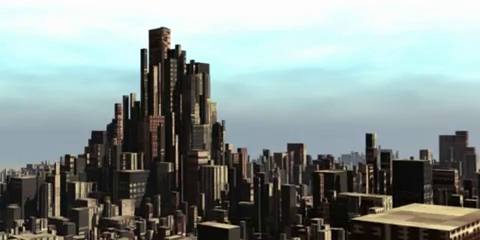
\includegraphics[width=0.7\textwidth]{images/shot0003.png}
  \caption{la ville de jour}
  \label{fig:villes1}
\end{figure}
\begin{figure}[h!]
  \centering

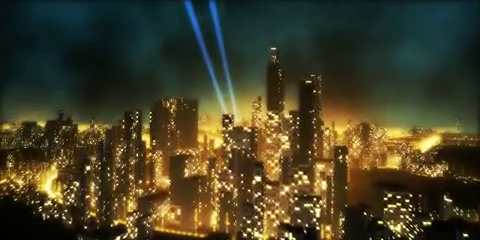
\includegraphics[width=0.7\textwidth]{images/shot0005.png}
  \caption{la ville de nuit}
  \label{fig:villes2}
\end{figure}
\begin{figure}[h!]
  \centering

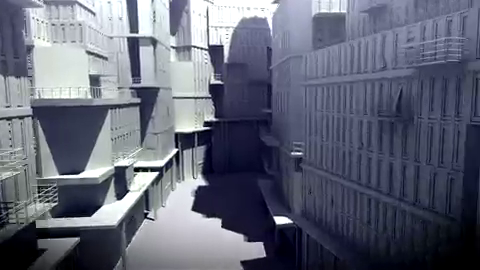
\includegraphics[width=0.7\textwidth]{images/shot0006.png}
  \caption{la ville de l'intérieur}
  \label{fig:villes3}
\end{figure}

\section*{sources}
Blender City Generator v0.4 :\\
\href{http://www.youtube.com/watch?v=HROU3gLcgfg&feature=related}{\url{http://www.youtube.com/watch?v=HROU3gLcgfg&feature=related}}\\

Building Generator v.01 flythrough :\\
\href{http://www.youtube.com/watch?v=N0LDnz-gq_o&NR=}{\url{http://www.youtube.com/watch?v=N0LDnz-gq_o&NR=}}\\


\end{document}
